\subsection{Management of Single-Resource Problems}
In the following, the approach for single-resource problems by \citet{klein2008} will be illustrated. \citet{klein2008} integrated the static capacity-based revenue management model ''Littlewood's Rule'' with overbooking methods. In the course of an extended formulation they implemented dynamic elements to Littlewood's Rule. Other approaches in \citet[Chapter 4]{talluri2004} combine class-allocation of quantity-based revenue management with overbooking methods.By doing this, they increased the level of detail by distinguishing between no-shows and cancellations. In addition to that, they further evaluate the static and dynamic dimension for no-shows and cancellations. In this paper only the approach by \citet{klein2008} will be explained due to its intuition.
\subsubsection{Single-Resource Management with a Decision Tree Model in accordance with \citet{bodily1995}}
In the following, model by \citet{bodily1995} will be described which is a modification of the rule of Littlewood. For this purpose, a short recap on the rule of Littlewood will be given at first. The following assumptions in accordance with \citet[p.86]{klein2008} shall hold for Littlewood's rule:
\begin{description}
	\item(i) The case of $n = 2$ products ($P_{1}$ and $P_{2}$) is considered.
	\item(ii) Revenues of $P_{1}$ are equal or higher then revenues of $P_{2}$: $r_{1}\geq r_{2}$.
	\item(iii) The amount of demand for products $P_{1}$ and $P_{2}$ is described via the random variables $D_{1}$ and $D_{2}$.
	\item(iv) Demand for $P_{2}$ arrives completely before demand for $P_{1}$.
	\item(v) The total capacity is expressed by $C$ in capacity units.
\end{description}
It is assumed that $x_{2}$ requests for $P_{2}$ have already arrived. The object of the decision-making situation results in the next incoming requests of $P_{2}$ $(x_{2}+1)$. The value of \textit{p} (see figure \ref{littlewood}) describes the probability that the sum of accepted requests for $P_{2}$ and additional upcoming requests for $P_{1}$ is smaller than the current available capacity \textit{C}:
\begin{equation}
p=P(x_{2}+D_{1}<C).
\end{equation}
A decision has to be made whether to accept the additional request for $P_{2}$ and therefore earning additional revenues of $r_{2}$ (upper half of figure \ref{littlewood}) or to deny the additional request for $P_{2}$ (bottom half of figure \ref{littlewood}) and to earn a revenue of $r_{1}$ with the probability $(1-p)$. The incoming request for $P_{2}$ will be accepted when: $p\geq\frac{r_{1}-r_{2}}{r_{1}}$.

\begin{figure}[h!]
	\begin{center}
		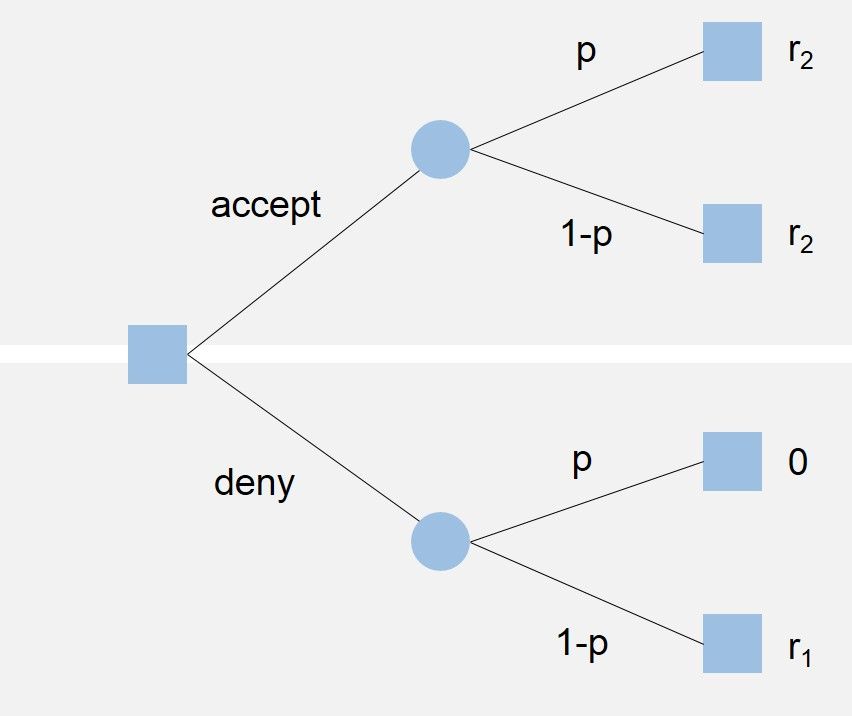
\includegraphics[width=0.5\textwidth]{littlewood.jpg}
		\label{littlewood}
		\caption{Capacity Control for Single-Flights in Accordance with \citet[p.162]{klein2008}} 
	\end{center}
\end{figure}	

Littlewood's rule was extended by \citet[p.176 ff.]{bodily1995} for solving simultaneously combined overcapacity and capacity control problems for single-resources (see figure \ref{littlewood1}). The following assumptions shall be added:
\begin{description}
	\item(vi) The random variables $S_{1}$ and $S_{2}$ define how many of the accepted requests of $P_{1}$ and $P_{2}$, respectively, will show-up until point of service.
	\item(vii)\label{vii_} All additional requests for $P_{1}$ will be accepted.
	\item(viii) The variable \textit{q} defines the probability that the additional request will turn up upon point of service.
	\item(viiii) The variable \textit{g} defines the costs of denied service.
\end{description}
In contrast to the previous formulation, the value of \textit{p} describes the probability that the sum of $S_{1}$ and $S_{2}$ will be smaller than the total capacity \textit{C}:
\begin{equation}
p=P(S_{1}+S_{2}<C).
\end{equation}
In this formulation, marginal revenues are illustrated. In the upper half of figure \ref{littlewood1}, assuming that $x_{2}$ requests for $P_{2}$ have already arrived and under condition (vii), the acceptance of an additional request for $P_{2}$ would generate additional marginal revenues $r_{2}$ because the capacity is not exhausted. On the bottom half, however, an acceptance of an additional demand of $P_{2}$ with no free capacity would result in increased marginal revenues minus the costs of denied service. The incoming request for $P_{2}$ will be accepted when: $p\geq\frac{g-r_{2}}{g}$\cite{bodily}.

\begin{figure}[h]
	\begin{center}
		\includegraphics[width=0.5\textwidth]{bild1.jpg}
		\label{littlewood1}
		\caption{Simultaneous Overbooking and Capacity Control Management for Single-Flights in Accordance with \citet[p.163]{klein2008}} 
	\end{center}
\end{figure}

%\subsection{Overbooking with class allocation in accordance with Talluri}
%The following assumptions in accordance with \citet[p.155]{talluri2004} shall hold for the illustration of different approaches in overbooking and capacity control:
%\begin{description}
%	\item(i) '' The cancellation and no-show probabilities are the same for all customers.''
%	\item(ii) '' Cancellations and no-shows are mutually independent across customers.''
%	\item(iii) '' Cancellations and no-shows in any period are independent of the time the reservations on hand were accepted.''
%	\item(iv) '' The refunds and denied-service costs are the same for all customers.''
%\end{description}